\chapter{Project Management}\label{app:management}
\section{Schedule and dependencies}
Figure~\ref{fig:gantt} separates recorded semester evidence from
forward delivery work. A marker indicates an
event or evidence date, not continuous effort or completed hours. Earlier
8/15 October prototype targets are retained as historical obligations; they
are not silently replaced by the November plan.

\begin{figure}[htbp]\centering
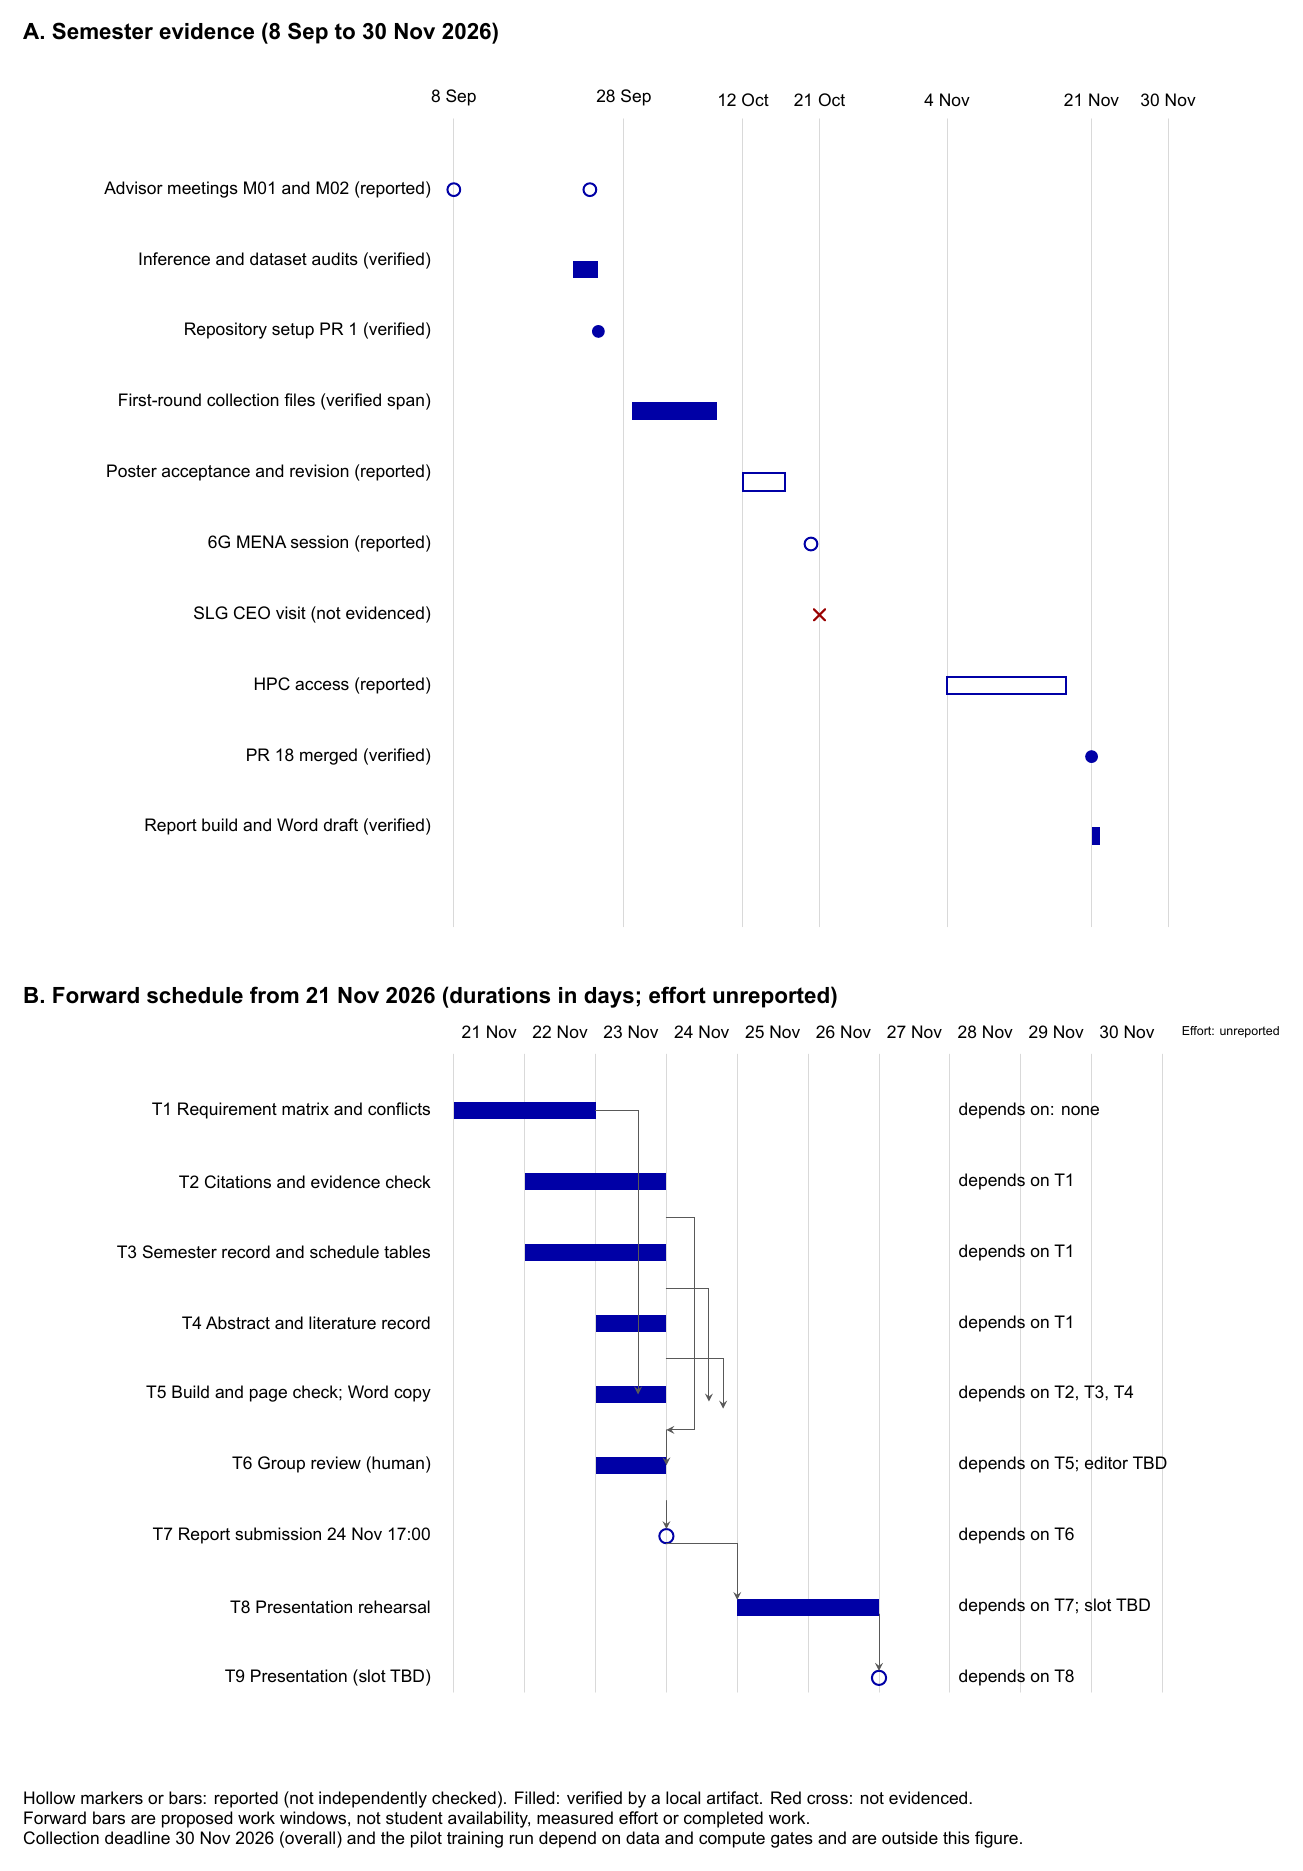
\includegraphics[width=\textwidth]{gantt.png}
\caption{Schedule summary in two panels. Panel A places recorded semester events by evidence status: filled markers are verified, hollow markers are reported and not independently checked, and the red cross is not evidenced. Panel B gives the forward schedule from 21 November 2026 with durations, dependencies and responsibilities. Effort is unreported for every task, and no bar measures student effort.}
\label{fig:gantt}
\end{figure}

\begingroup\small
\begin{longtable}{p{0.21\textwidth}p{0.34\textwidth}p{0.35\textwidth}}
\caption{Dependencies and contingencies for the final SDP I delivery.}\\
\toprule Deliverable & Required dependency & Contingency or open action\\\midrule\endfirsthead
\toprule Deliverable & Required dependency & Contingency or open action\\\midrule\endhead
Training pilot & Reviewed data receipts, actual initialization and qualified backend & Report software preparation and precise blockers if execution cannot qualify\\
Real evaluation & Matching predictions/ground truth and frozen protocol & Keep results explicitly unavailable; never substitute paper or synthetic scores\\
Demo & Current machine, engine/model identity and authorized examples & Clearly labeled saved real-run fallback, with known failures retained\\
Report & Verified evidence, reference review, forms and student contribution statements & Freeze factual content for 23 Nov review; retain explicit limitations\\
Submission & Active Blackboard format, project number, actual signatures and distribution clearance & Checked Word copy alongside LaTeX PDF; confirm institutional instructions before upload\\
Distributed work & QC, accepted counts, labels and physical/case grouping & Preserve 30 Nov collection obligation; do not infer P2 completion\\\bottomrule
\end{longtable}
\endgroup

Task names identify coordination contacts, not exclusive rights to files.
Students prioritize assigned work and may complete a small dependency that
blocks it without waiting for its lead. They record actual editor/scope and
coordinate overlapping active edits or GPU/output use. Independent review
and truthful credit remain necessary. The sole live backlog is
\file{docs/tasks.md}; this appendix is a dated summary.

\section{Semester record}
Table~\ref{tab:record} lists events and milestones from September to November 2026.
Each row states its evidence status. \emph{Verified} means a local artifact, repository
state or read-back confirms it. \emph{Reported} means an owner statement, email or meeting
record that has not been independently checked. Conflicts are listed in
Table~\ref{tab:conflicts} and are not resolved here.

\begingroup\small
\begin{longtable}{>{\raggedright\arraybackslash}p{0.14\textwidth}>{\raggedright\arraybackslash}p{0.36\textwidth}>{\raggedright\arraybackslash}p{0.22\textwidth}>{\raggedright\arraybackslash}p{0.18\textwidth}}
\caption{Dated semester record, September to November 2026.}\label{tab:record}\\
\toprule Date & Event & Outcome & Evidence\\\midrule\endfirsthead
\toprule Date & Event & Outcome & Evidence\\\midrule\endhead
8 Sep 2026 & Advisor meeting M01 (Prof.\ Werghi) & Source minutes and companion; attendance not confirmed & Reported\\
22--25 Sep & Generic inference and dataset audits & Generic inference ran; device-label and split findings recorded & Verified\\
24 Sep & Advisor meeting M02; Divya follow-up F02 & Batch 1 by 15 Oct, Batch 2 after midterms, GUI and poster tasks & Reported (minutes hash verified)\\
25 Sep & Team repository setup (PR \#1, rulesets) & Published; hosted checks passed & Verified\\
28 Sep & Collection emails F03--F05; catalogue C01 & Revised slots 29 Sep--8 Oct; catalogue structure checked & Reported; catalogue verified\\
29 Sep--9 Oct & First-round collection files (filename span only) & 577 JPEG paths, 478 distinct payloads, all decode & Verified (files); sessions reported\\
12--17 Oct & Poster acceptance and revision & Accepted 12 Oct; revised file 17 Oct; TDRA response pending & Reported\\
19 Oct & Collection update F06; SLG visit invitation F08 & 30 Nov overall deadline; visit 21 Oct, 14:00--17:00 & Reported (invitation only)\\
20 Oct & 6G MENA session, Abu Dhabi & Team attendance owner-reported; presentation evidence not reviewed & Reported\\
21 Oct & SLG CEO visit & No outcome recorded in the project record & Not evidenced\\
4--18 Nov & CS-HPC access email; owner confirmation & Access issued; training run not verified & Reported\\
21 Nov & PR \#18 merged (commit 9350482) & 273 evaluation-enabled tests and required CI passed & Verified\\
21 Nov & Report LaTeX build and Word draft & Local build passes; Word layout review open & Verified (local)\\bottomrule
\end{longtable}
\endgroup

\textbf{Conferences and events.} The project record lists the ISDIA and ICISAS calls
(closed 15 November 2026, no submission recorded), the CVCI call (official deadline
30 November 2026, conflicting with a 5 December invitation) and a ZU SRC abstract window
(15 December 2026 to 18 January 2027). No submission or acceptance for any event is recorded.

\begingroup\small
\begin{longtable}{>{\raggedright\arraybackslash}p{0.44\textwidth}>{\raggedright\arraybackslash}p{0.52\textwidth}}
\caption{Open conflicts recorded in the project, not resolved in this report.}\label{tab:conflicts}\\
\toprule Item & Conflict\\\midrule\endfirsthead
\toprule Item & Conflict\\\midrule\endhead
Report deadline & 24 Nov 2026, 17:00 UTC+4 (owner) versus 27 Nov 2026 (pasted notice)\\
Collection deadline & Batch 1 by 15 Oct (historical) versus 30 Nov overall\\
Collection count & Target 500 versus 577 paths and 478 distinct payloads\\
Round 1 allocation & One item per student (F03) versus all four families per student (C01)\\
PR \#21 status & Recorded as merged in one task row and open in the status record\\
Logo adoption & A04 in one progress heading versus A03 approved 28 Sep in the status record\\
Poster timeline & 30 Sep, 14 Oct, 17 Oct revision versus 20 Oct confirmation\\
\bottomrule
\end{longtable}
\endgroup

\section{Handbook-form task schedule}
Table~\ref{tab:tasks} sets out the schedule elements the handbook asks for. Effort in hours
was not recorded for any task, so the effort column reads ``unreported'' rather than an estimate.
Durations are the dates in the project record, not measured effort.

\begingroup\small
\begin{longtable}{>{\raggedright\arraybackslash}p{0.22\textwidth}>{\raggedright\arraybackslash}p{0.10\textwidth}>{\raggedright\arraybackslash}p{0.12\textwidth}>{\raggedright\arraybackslash}p{0.26\textwidth}>{\raggedright\arraybackslash}p{0.22\textwidth}}
\caption{Task schedule in handbook form (effort unreported).}\label{tab:tasks}\\
\toprule Task & Duration & Effort & Depends on & Output and contingency\\\midrule\endfirsthead
\toprule Task & Duration & Effort & Depends on & Output and contingency\\\midrule\endhead
Report drafting (LaTeX, bibliography) & 21--24 Nov & unreported & Verified evidence; references & Build and PDF; contingency: freeze content for review\\
Group review and Word copy & 23--24 Nov & unreported & Build; Pandoc conversion & Word draft; contingency: PDF if accepted\\
Presentation rehearsal & 25--26 Nov & unreported & Demo candidate; slot & Rehearsed demo; contingency: recorded fallback\\
Presentation & 27 Nov (stated) & unreported & Slot confirmation & Presentation; slot TBD\\
Collection completion & to 30 Nov & unreported & Lab protocol; QC & Accepted counts; open conflict in Table~\ref{tab:conflicts}\\
Pilot training and evaluation & after data gates & unreported & Data receipts; qualified runtime & Not started; no results claimed\\bottomrule
\end{longtable}
\endgroup

\chapter{Risk and Required Forms}\label{app:risk}
\section{Risk preparation worksheet}
Table~\ref{tab:risk} is a draft engineering worksheet for discussion, not the
official completed Risk Assessment or Health and Safety form. Likelihood,
severity, residual ratings and named signatories require supervisor/lab review.
No signature, approval or absence of hazards is inferred here.

\begingroup\small
\begin{longtable}{p{0.2\textwidth}p{0.32\textwidth}p{0.38\textwidth}}
\caption{Draft hazard and project-risk discussion worksheet.}\label{tab:risk}\\
\toprule Hazard or risk & Possible consequence & Proposed controls and outstanding review\\\midrule\endfirsthead
\toprule Hazard or risk & Possible consequence & Proposed controls and outstanding review\\\midrule\endhead
Lab X-ray equipment & Exposure or unsafe operation & Trained authorized operation, intact interlocks and lab procedures; lab/supervisor determines applicable radiation controls\\
Electrical equipment and specimen handling & Injury, damage or unapproved operation & Follow lab-approved equipment/specimen protocol; no unsupervised hazardous work; confirm permitted inert materials with lab\\
Missed detections or overconfidence & Incorrect inspection decision & Human review, known-miss demonstration, visible failure states and no safe verdict from empty results\\
Data and credentials & Disclosure or unauthorized access & Authorized local storage, sanitized exports, no scans/weights/credentials/private paths in public Git\\
Split leakage and invalid labels & Misleading evaluation or tuning & Preserve published test, hash artifacts, group duplicates, review geometry and physical provenance; no test-based tuning\\
Compute failure or excess resource use & Lost study evidence, missed deadline or quota breach & One job/output owner, checkpoint/restart evidence, bounded pilot and measured budget before search\\
Software mismatch & Invalid result or demo failure & Pinned environments, actual device/revision records, clean startup checks and labeled recorded fallback\\
Contribution and AI attribution & Misrepresentation in individual assessment & Actual work links, student explain-back and truthful assistance disclosure; no invented hours\\
Report and publication & Rejected submission or confidential disclosure & Confirm Word/PDF acceptance and filename; actual form signatures; resolve written-permission requirement before public distribution\\\bottomrule
\end{longtable}
\endgroup

\section{Official form insertion checklist}
The handbook lists Risk Assessment and Health and Safety forms for SDP I/II.
Its Health and Safety form calls for student representative and supervisor
signatures and handling by the University Safety Officer. Confirm the current
course templates and insert their completed, authorized copies into the
submission version. Do not mark the project software-only without reviewing
the team's physical lab collection work.

\pending{Official Risk Assessment form, completed Health and Safety form,
current declaration wording, actual signatures, recipients and dates. The
current draft intentionally contains no fabricated declaration or signature.}

The Project Clearance I/II forms are explicitly marked for the SDP II final
report. They are not treated as new SDP I submission requirements without
a specific course instruction. Physical final-copy requirements and public
distribution remain to be clarified against the later course notices.

\chapter{Contribution and Assistance Record}\label{app:contributions}
The entries below distinguish repository evidence from personal understanding.
They are draft source records for student confirmation, not a final allocation
of marks or hours. Team names follow shared records and require roster confirmation.

\begingroup\small
\begin{longtable}{p{0.19\textwidth}p{0.41\textwidth}p{0.3\textwidth}}
\caption{Evidence-linked contribution worksheet for individual confirmation.}\\
\toprule Student & Existing source record & Verification still needed\\\midrule\endfirsthead
\toprule Student & Existing source record & Verification still needed\\\midrule\endhead
Abd Alrahman Ismaik & Coordination/GUI direction recorded in project documentation; assisted integration and report preparation & Personal reviewed contribution statement, report sections and explain-back\\
Faisal Daoud Alzarooni & T40 baseline/contracts/tools PRs 17/19; initialization PR 21 & Student confirmation, actual HPC handoff and explain-back\\
Ahmed Almansoori & T41 branch commit 32091bc; pipeline checks, planning and synthetic study draft & Student confirmation and integration evidence; real training not yet established\\
Ali Arif Alshamsi & T42 evaluator PR 18, validation interface and matched comparison & Student confirmation, real evaluation evidence when available and explain-back\\
Mohammad Arwani & Research branch records an assisted app acceptance slice & Verified shared app commit/diff, human walkthrough and roster spelling\\\bottomrule
\end{longtable}
\endgroup

AI assistance was used in implementation, review and documentation preparation,
including this report draft. Each student must review and understand the work
they claim. Relevant sanitized code-generation prompts and assistance details
must be included accurately in the final disclosure; private transcripts,
credentials and session records remain outside the public repository.
\pending{Student-reviewed disclosure and relevant sanitized prompt excerpts.}

\chapter{Handbook Coverage and Source Map}\label{app:coverage}
\begingroup\small
\begin{longtable}{p{0.12\textwidth}p{0.45\textwidth}p{0.33\textwidth}}
\caption{R01--R15 traceability for this draft. Presence is not final acceptance.}\\
\toprule ID & Draft location & Remaining gate\\\midrule\endfirsthead
\toprule ID & Draft location & Remaining gate\\\midrule\endhead
R01 & Cover, abstract, contents and lists & Institutional cover/roster confirmation\\
R02 & Chapter 1 objectives and scope & Student/supervisor review\\
R03 & Chapter 1 literature & Deeper reference reading; scoped patent-search record\\
R04 & Chapter 1 and Appendix C & Individual confirmations and sanitized prompts\\
R05 & Chapter 2, Table 2.1 & Formal requirements/specification review\\
R06 & Chapter 3 & Technical review of assumptions and equations\\
R07 & Chapter 4 & Final design rationale review\\
R08 & Chapter 5 & Current app revision and approved screenshots\\
R09 & Chapter 5 & Eligible real metrics and demonstration evidence\\
R10 & Chapter 6 & Conclusions updated to final evidence cutoff\\
R11 & References & Verify relevance, metadata and final citation coverage\\
R12 & Appendix A and original specification below & Gantt actuals/student ownership confirmation\\
R13 & Appendix B & Official completed forms and actual signatures\\
R14 & Appendix B & Official declaration and applicable paperwork\\
R15 & Project course checklist & Actual submission, permission and rehearsal receipts\\\bottomrule
\end{longtable}
\endgroup

\section{Original specification summary}
The original proposal requires image acquisition of 500 positive/negative
samples; preprocessing for image quality; contemporary explosive detection;
evaluation on unseen test data; and a GUI supporting control and recording.
This summary preserves the requirements without reproducing private source
documents. Later meetings prioritize distributed collection and retain a
single-scan existing-model showcase. Table~\ref{tab:requirements} maps the
current implementation without treating later planning as waiver of older
requirements.

\section{Project source register}
\begingroup\small
\begin{longtable}{p{0.4\textwidth}p{0.5\textwidth}}
\caption{Project records supporting the report; paths are repository-relative.}\\
\toprule Source record & Use and evidence boundary\\\midrule\endfirsthead
\toprule Source record & Use and evidence boundary\\\midrule\endhead
\file{docs/final-report-requirements.md} & Handbook requirements and R01--R15; original handbook remains local\\
\file{docs/meeting_minutes/README.md} & M01/M02 and F02--F08 directions; minutes do not prove execution\\
\file{docs/research.md} & Paper and release inspection; published claims remain distinct\\
\file{docs/iedxray-audit.md} & Audit findings and source preservation\\
\file{docs/first-inference.md} & Initial executed CPU diagnostic inference and retained miss\\
\file{docs/architecture.md} & Contract and repository boundary; older passages require revision-aware reading\\
\file{docs/collection-progress-2026-11-14.md} & Path/byte inventory and unresolved QC/provenance\\
\file{docs/progress.md} & Dated integration commands, test outcomes and limitations\\
\file{docs/course-endgame-2026-11.md} & Submission/presentation notices and conflicts\\
\file{docs/tasks.md} & Sole live backlog; this report is a dated evidence snapshot\\\bottomrule
\end{longtable}
\endgroup
